\chapter{Results}
\label{ch:6}

In this chapter, we will present the results of the analysis we conducted.
First, we briefly look at how the algorithms scored the trajectories. 
For the remainder of the chapter, we focus on the clusters and meaningfully interpret them. 



\section{Similarity Scores}
Even though they lay the basis for further analysis, there is no meaningful way to directly compare the similarity scores. 
However, it could be interesting to look at their ranking of trajectory pairs. 
We are present the ten pairs that each measure deemed the most similar in \Cref{tab:top-10-sim-pairs}. 

\begin{table}[]
\centering
\caption{Overview of most similar trajectory pairs according to each measure. A larger version of the table is in\Cref{app:a-simtab}  }
\resizebox{\textwidth}{!}{%
\renewcommand{\arraystretch}{1.1}
\begin{tabular}{@{}|l|l|l|l|l|l|l|l|l|l|@{}}
\toprule
\textbf{Euclidean} &
  \textbf{DTW} &
  \textbf{SSPD} &
  \textbf{Hausdorff} &
  \textbf{ERP} &
  \textbf{MSM; cost=1} &
  \textbf{MSM; cost=.1} &
  \textbf{MSM; cost=.01} &
  \textbf{EDR; $\epsilon=.203$} &
  \textbf{EDR; $\epsilon=.101$} \\ \midrule
{\color[HTML]{CB0000} \textit{QREOR-IHNMX}} &
  {\color[HTML]{986536} \textit{LFQDH-ACJIG}} &
  {\color[HTML]{986536} \textit{LFQDH-ACJIG}} &
  {\color[HTML]{000000} WBNSL-SATNK} &
  {\color[HTML]{CB0000} \textit{QREOR-IHNMX}} &
  {\color[HTML]{CB0000} \textit{QREOR-IHNMX}} &
  {\color[HTML]{CB0000} \textit{QREOR-IHNMX}} &
  {\color[HTML]{986536} \textit{LFQDH-ACJIG}} &
  {\color[HTML]{986536} \textit{LFQDH-ACJIG}} &
  {\color[HTML]{986536} \textit{LFQDH-ACJIG}} \\
{\color[HTML]{986536} \textit{LFQDH-ACJIG}} &
  {\color[HTML]{009901} \textit{NVZCQ-TGKDX}} &
  {\color[HTML]{000000} WBNSL-SATNK} &
  {\color[HTML]{009901} \textit{NVZCQ-TGKDX}} &
  {\color[HTML]{986536} \textit{LFQDH-ACJIG}} &
  {\color[HTML]{986536} \textit{LFQDH-ACJIG}} &
  {\color[HTML]{986536} \textit{LFQDH-ACJIG}} &
  {\color[HTML]{009901} \textit{NVZCQ-TGKDX}} &
  {\color[HTML]{000000} LVFYZ-LENWX} &
  {\color[HTML]{CB0000} \textit{QREOR-IHNMX}} \\
{\color[HTML]{000000} BZCYT-VXLBC} &
  {\color[HTML]{CB0000} \textit{QREOR-IHNMX}} &
  {\color[HTML]{000000} KQQUG-OVNBK} &
  {\color[HTML]{000000} NHNMB-PSVVR} &
  {\color[HTML]{000000} BZCYT-VXLBC} &
  {\color[HTML]{000000} BZCYT-VXLBC} &
  {\color[HTML]{009901} \textit{NVZCQ-TGKDX}} &
  {\color[HTML]{000000} KQQUG-OVNBK} &
  {\color[HTML]{000000} XXVQK-LOBQA} &
  {\color[HTML]{000000} KQQUG-OVNBK} \\
{\color[HTML]{3531FF} \textit{LHTXJ-TGKDX}} &
  {\color[HTML]{000000} HXVAH-RPCOW} &
  {\color[HTML]{CB0000} \textit{QREOR-IHNMX}} &
  {\color[HTML]{000000} HXVAH-RPCOW} &
  {\color[HTML]{3531FF} \textit{LHTXJ-TGKDX}} &
  {\color[HTML]{3531FF} \textit{LHTXJ-TGKDX}} &
  {\color[HTML]{000000} BZCYT-VXLBC} &
  {\color[HTML]{000000} WBNSL-SATNK} &
  {\color[HTML]{000000} BLHVW-ATPTV} &
  {\color[HTML]{000000} LFQDH-ASYEZ} \\
{\color[HTML]{000000} PSVVR-XSJJE} &
  {\color[HTML]{000000} KQQUG-OVNBK} &
  {\color[HTML]{000000} NHNMB-PSVVR} &
  {\color[HTML]{CB0000} \textit{QREOR-IHNMX}} &
  {\color[HTML]{000000} PSVVR-XSJJE} &
  {\color[HTML]{000000} PSVVR-XSJJE} &
  {\color[HTML]{000000} KQQUG-OVNBK} &
  {\color[HTML]{CB0000} \textit{QREOR-IHNMX}} &
  {\color[HTML]{000000} WBTAG-QMRPP} &
  {\color[HTML]{009901} \textit{NVZCQ-TGKDX}} \\
{\color[HTML]{009901} \textit{NVZCQ-TGKDX}} &
  {\color[HTML]{000000} JRDIM-OVNBK} &
  {\color[HTML]{009901} NVZCQ-TGKDX} &
  {\color[HTML]{000000} JRDIM-OVNBK} &
  {\color[HTML]{009901} \textit{NVZCQ-TGKDX}} &
  {\color[HTML]{009901} \textit{NVZCQ-TGKDX}} &
  {\color[HTML]{000000} LFQDH-ASYEZ} &
  {\color[HTML]{000000} HXVAH-RPCOW} &
  {\color[HTML]{000000} NKEGR-VXLBC} &
  {\color[HTML]{000000} BZCYT-VXLBC} \\
{\color[HTML]{000000} TNPJQ-LRZLR} &
  {\color[HTML]{000000} WBNSL-SATNK} &
  {\color[HTML]{000000} HXVAH-RPCOW} &
  {\color[HTML]{986536} \textit{LFQDH-ACJIG}} &
  {\color[HTML]{000000} TNPJQ-LRZLR} &
  {\color[HTML]{000000} TNPJQ-LRZLR} &
  {\color[HTML]{3531FF} \textit{LHTXJ-TGKDX}} &
  {\color[HTML]{3531FF} \textit{LHTXJ-TGKDX}} &
  {\color[HTML]{000000} TNPJQ-LRZLR} &
  {\color[HTML]{000000} PSVVR-XSJJE} \\
{\color[HTML]{000000} HUSJF-UHLAI} &
  {\color[HTML]{000000} NHNMB-PSVVR} &
  {\color[HTML]{000000} JRDIM-OVNBK} &
  {\color[HTML]{000000} KQQUG-OVNBK} &
  {\color[HTML]{000000} HUSJF-UHLAI} &
  {\color[HTML]{000000} HUSJF-UHLAI} &
  {\color[HTML]{000000} PSVVR-XSJJE} &
  {\color[HTML]{000000} JRDIM-OVNBK} &
  {\color[HTML]{000000} PSVVR-XSJJE} &
  {\color[HTML]{000000} KQQUG-GRPNX} \\
{\color[HTML]{000000} ZQZSA-NVZCQ} &
  {\color[HTML]{3531FF} \textit{LHTXJ-TGKDX}} &
  {\color[HTML]{3531FF} \textit{LHTXJ-TGKDX}} &
  {\color[HTML]{000000} DADNP-LOBQA} &
  {\color[HTML]{000000} ZQZSA-NVZCQ} &
  {\color[HTML]{000000} ZQZSA-NVZCQ} &
  {\color[HTML]{000000} HXVAH-RPCOW} &
  {\color[HTML]{000000} LFQDH-ASYEZ} &
  {\color[HTML]{3531FF} \textit{LHTXJ-TGKDX}} &
  {\color[HTML]{000000} CWCGU-ACJIG} \\
{\color[HTML]{000000} NVZCQ-TNPJQ} &
  {\color[HTML]{000000} BZCYT-VXLBC} &
  {\color[HTML]{000000} SATNK-FIVOK} &
  {\color[HTML]{000000} OAAYX-OKPGU} &
  {\color[HTML]{000000} NVZCQ-TNPJQ} &
  {\color[HTML]{000000} NVZCQ-TNPJQ} &
  {\color[HTML]{000000} HUSJF-UHLAI} &
  {\color[HTML]{000000} NHNMB-PSVVR} &
  {\color[HTML]{000000} HUSJF-UHLAI} &
  {\color[HTML]{000000} EBYMF-LENWX} \\ \midrule
\end{tabular}
}
\label{tab:top-10-sim-pairs}
\end{table}


We observe that there is variance with respect to where the pairs are placed, yet there are a handful of recurrent pairs.
We noticed that one of the trajectory pairs appeared in the top-10 ranks for all the measures. 
Furthermore, two pairs appeared for all but one measure, and one pair that was in all but two. 
These four frequent pairs have been highlighted in \Cref{tab:top-10-sim-pairs} and are displayed in \Cref{fig:most_common_pairs}. 
The table has 27 distinct trajectory pairs, indicating that the measures generally agree on which pairs are the most similar ones. 

\begin{figure}[ht]
  \centering
  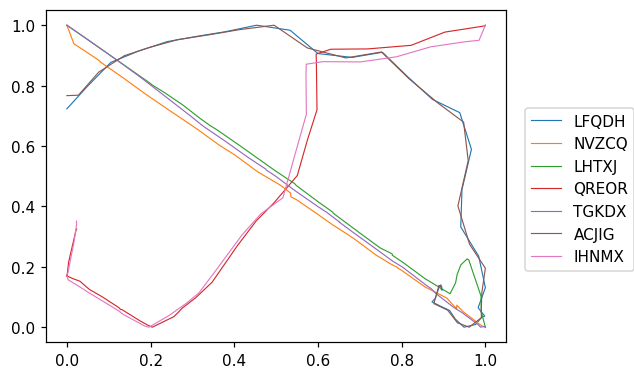
\includegraphics[width=.6\linewidth]{figs/traj/4_most_common.png}
  %    \begin{subfigure}[c]{0.35\linewidth}
  \caption{The trajectory pairs that appeared the most based on the similarity scores. }
  \label{fig:most_common_pairs}
\end{figure}




% in FIGURE the trajectories of the pairs that were the most frequent is shown. The left side has is the re-scaled tracks and the right ones is the raw GPS data.   


% \begin{table}[tbp]
%   \centering
%   \caption{Table of the top 10 most similar trajectory pairs}
%   \label{tab:top10}
%   \csvautobooktabular{csvtables/ageiq.csv}
% %   \csvautobooktabular{csvtables/TOP_10_ALL.csv}
% \end{table}


\section{Davies-Bouldin Index}

In \Cref{tab:cluster-dbidx} we have presented the Davies-Bouldin results for each cluster per type of clustering method. 
As was brought up in \Cref{ch:5} and further elaborated upon in \Cref{ch:7}, this is not a decisive ranking.


Three observations stand out in \Cref{tab:cluster-dbidx}.
Firstly, we note that SSPD and HD have received the worst ranks under both AP and HCA. 
Next, we remarked that Ed and MSM- which had identical rankings of trajectory pair, also got the same DB-index under both types of clustering.
ERP,  which also had an identical top-10 raking, received a DB-index under AP-clustering, but did so under HCA. 
The last thing that stands out is that the HCA gave a worse result for almost all methods, except for DTW and MSM with the lowest cost value. The difference is not significant, but it is consistent.


\begin{table}[h!]
\centering
\caption{Davies-Bouldin Indices for each cluster result and how each algorithm rank against each other according to this evaluation  }
\renewcommand{\arraystretch}{1.1}
\begin{tabular}{|c|	c|c|c|c|} 
\cline{2-5}
\multicolumn{1}{c|}{} & \multicolumn{2}{c|}{\textbf{Affinity Propagation}} & \multicolumn{2}{c|}{\textbf{Hierarchical Clustering}}  \\ 
\cline{2-5}
\multicolumn{1}{c|}{} & \textit{Score} & \textit{Rank}  & \textit{Score} & \textit{Rank}     \\ 
\hline
\textbf{Ed}           & 0.091 & 3    & 0.095 & 2        \\ 
\hline
\textbf{DTW}          & 0.156 & 8    & 0.140 & 5        \\ 
\hline
\textbf{Hd}           & 0.294 & 9    & 0.459 & 9        \\ 
\hline
\textbf{SSPD}         & 0.431 & 10   & 0.531 & 10       \\ 
\hline
\textbf{ERP}    & 0.083 & 2    & 0.090 & 1        \\ 
\hline
\textbf{EDR} $\epsilon=0.203$  & 0.082 & 1    & 0.162 & 6        \\ 
\hline
\textbf{EDR} $\epsilon=0.101$  & 0.091 & 3    & 0.217 & 7        \\ 
\hline
\textbf{MSM} cost$=0.01$   & 0.150 & 6    & 0.137 & 4        \\ 
\hline
\textbf{MSM} cost$=0.1$    & 0.155 & 7    & 0.222 & 8        \\ 
\hline
\textbf{MSM} cost$=1$      & 0.091 & 3    & 0.095 & 2        \\
\hline
\end{tabular}
\label{tab:cluster-dbidx}
\end{table}



\section{Clustering}

We restate that the area of interest for this thesis is the similarity distance measures and not various clustering techniques. 
The clusters are presented grouped by how they evaluated the trajectories' similarity, or by the underlying idea trajectory similarity. 

The two models used to create the clusters will be presented alongside each other.
The number of clusters produced under affinity propagation varied from 23 to 48, and as explained in \Cref{ch:5} the number of hierarchical clusters was set to 23 for all measures. See \Cref{app:ap-clu,app:h-clu} for higher resolution depictions of all clusters. 


The first three measures’ clusters we present are the ones with the identical ranking of most similar trajectory pairs;
Euclidean distance, ERP, and MSM with cost parameter to 1. The clusters are depicted in \Cref{fig:cluster-ed-erp-msm}. Next, \Cref{fig:cluster-msm} displays the clusters obtained from the remaining parameter values of Move-Split-Merge.
Continuing with the parameters measured, \Cref{fig:cluster-edr} shows the clusters that EDR generated with both parameter values. 
Finally, \Cref{fig:cluster-dtw-hd-sspd} shows the rest of the measures, namely clusters created with DTW, Hausdorff distance, and SSPD.



\begin{figure}[h]
  \centering
  \begin{subfigure}[c]{0.3\linewidth}
    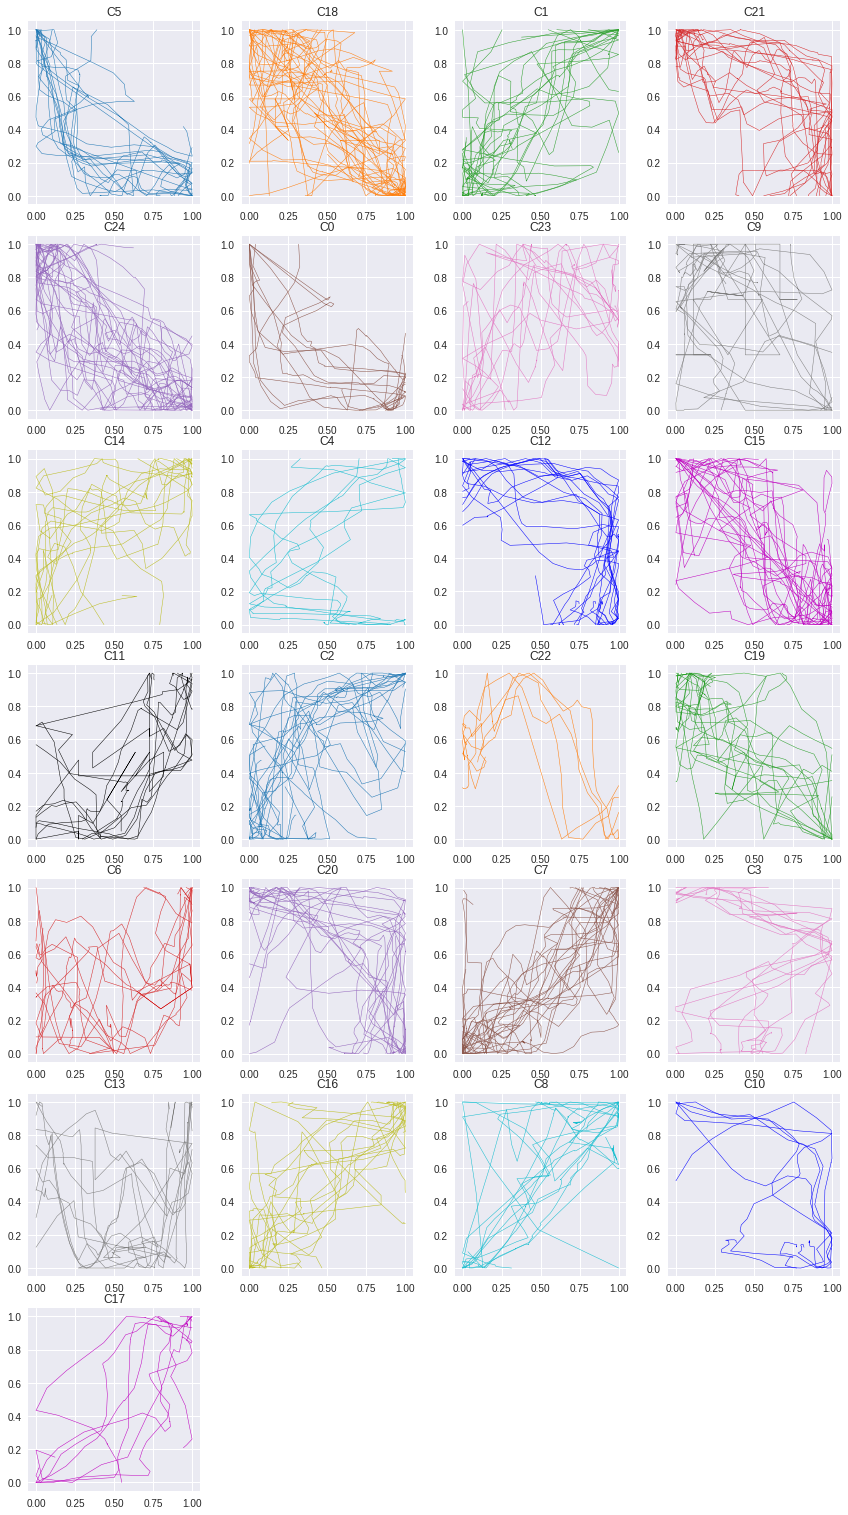
\includegraphics[width=\linewidth]{figs/clusters/CLU_AP_ALL[Ed].png}
    \caption{Euclidean}
  \end{subfigure}
  \hspace{.5em}
   \begin{subfigure}[c]{0.3\linewidth}
     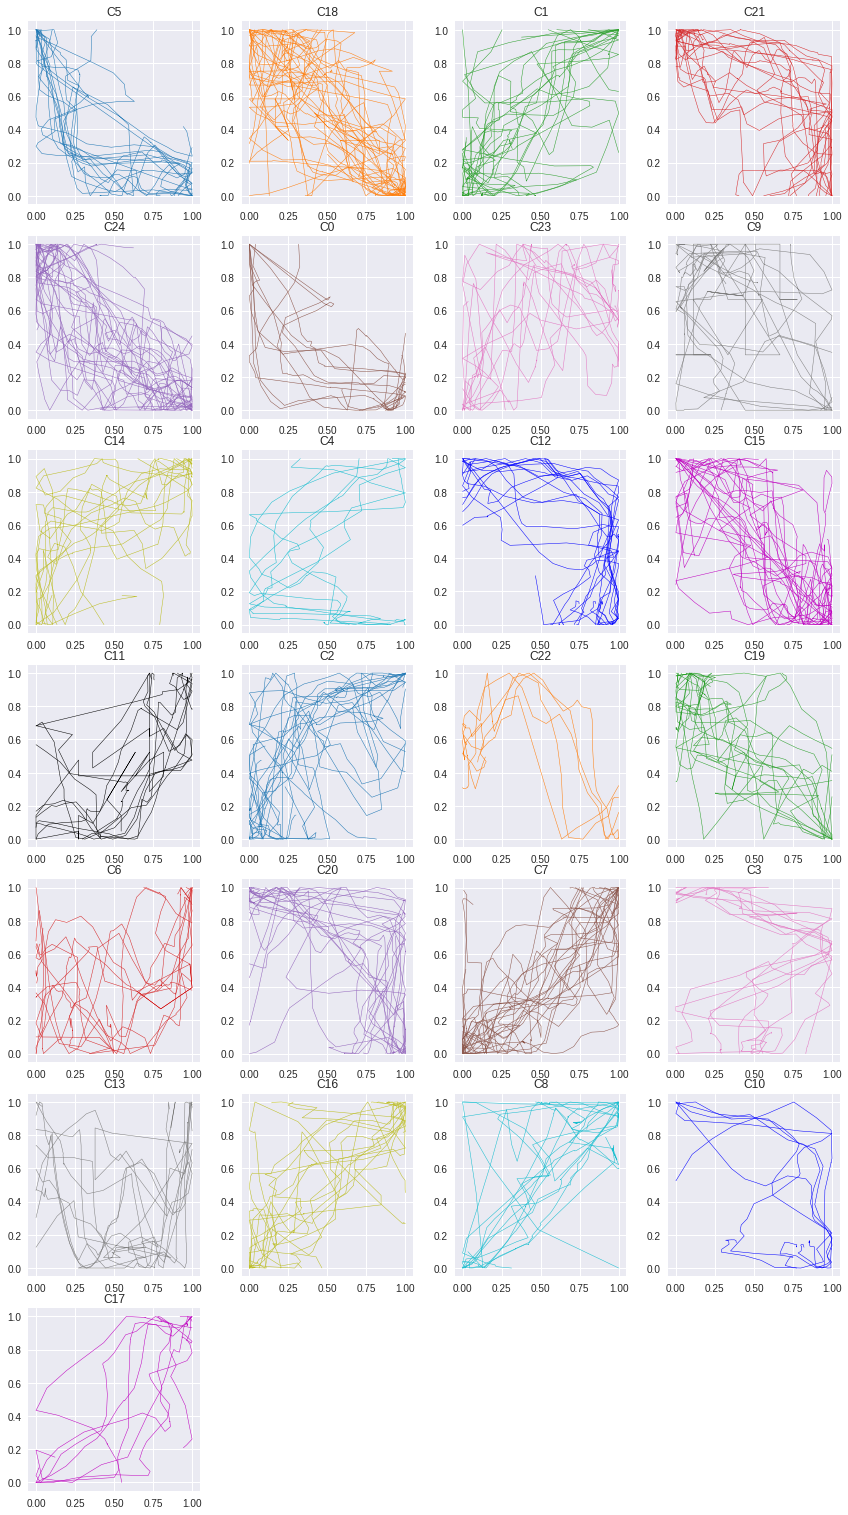
\includegraphics[width=\linewidth]{figs/clusters/CLU_AP_ALL[MSM;c=1].png}
    \caption{MSM; cost=1}
  \end{subfigure}
  \hspace{.5em}
    \begin{subfigure}[c]{0.3\linewidth}
     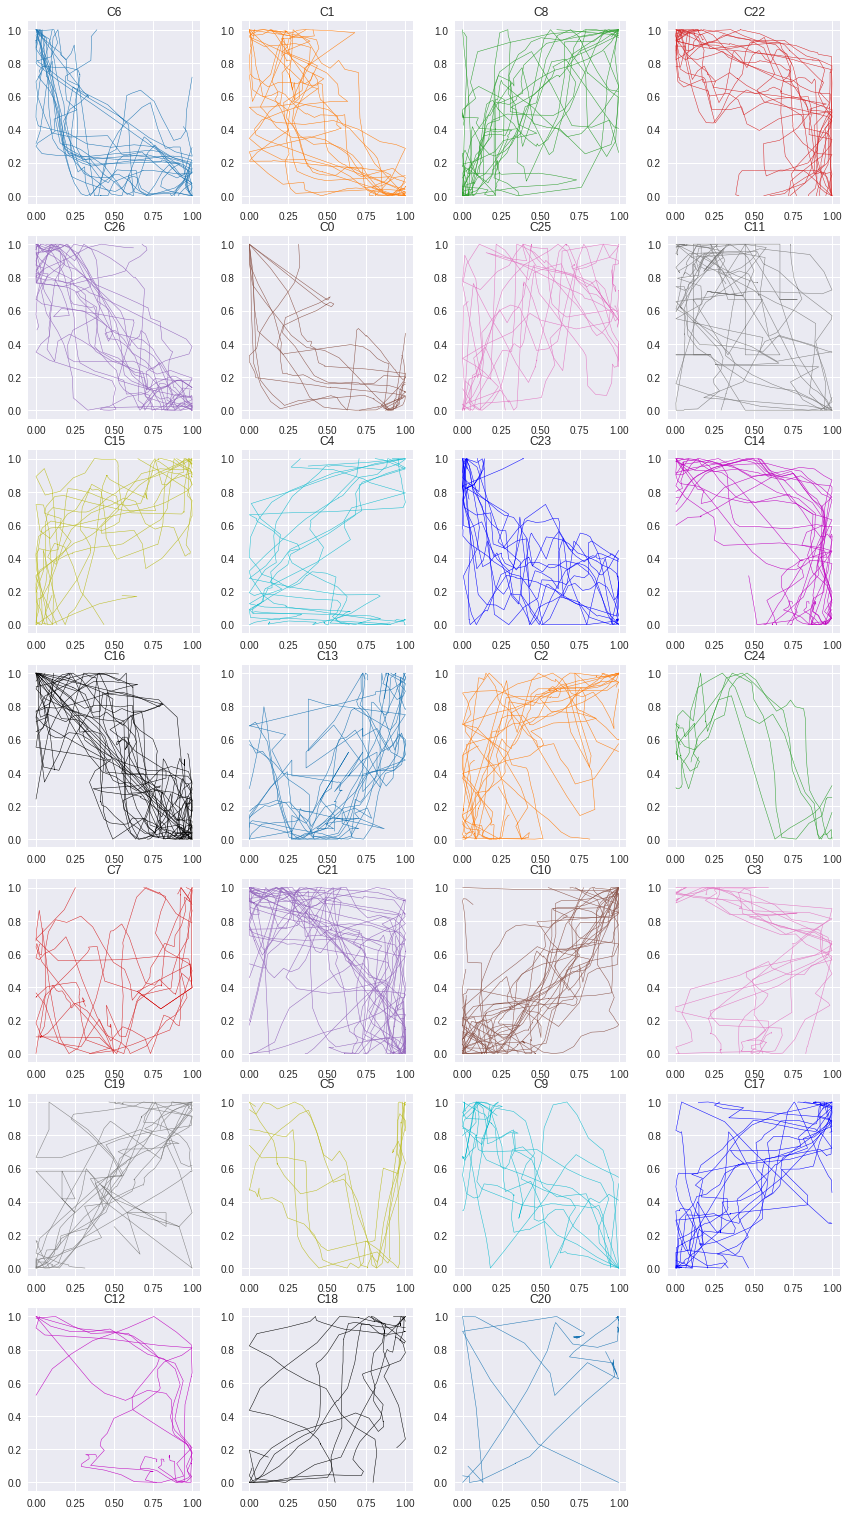
\includegraphics[width=\linewidth]{figs/clusters/CLU_AP_ALL[ERP;g=0,0].png}
    \caption{ERP}
  \end{subfigure}
  \hspace{.5em}
  
  \begin{subfigure}[c]{0.3\linewidth}
    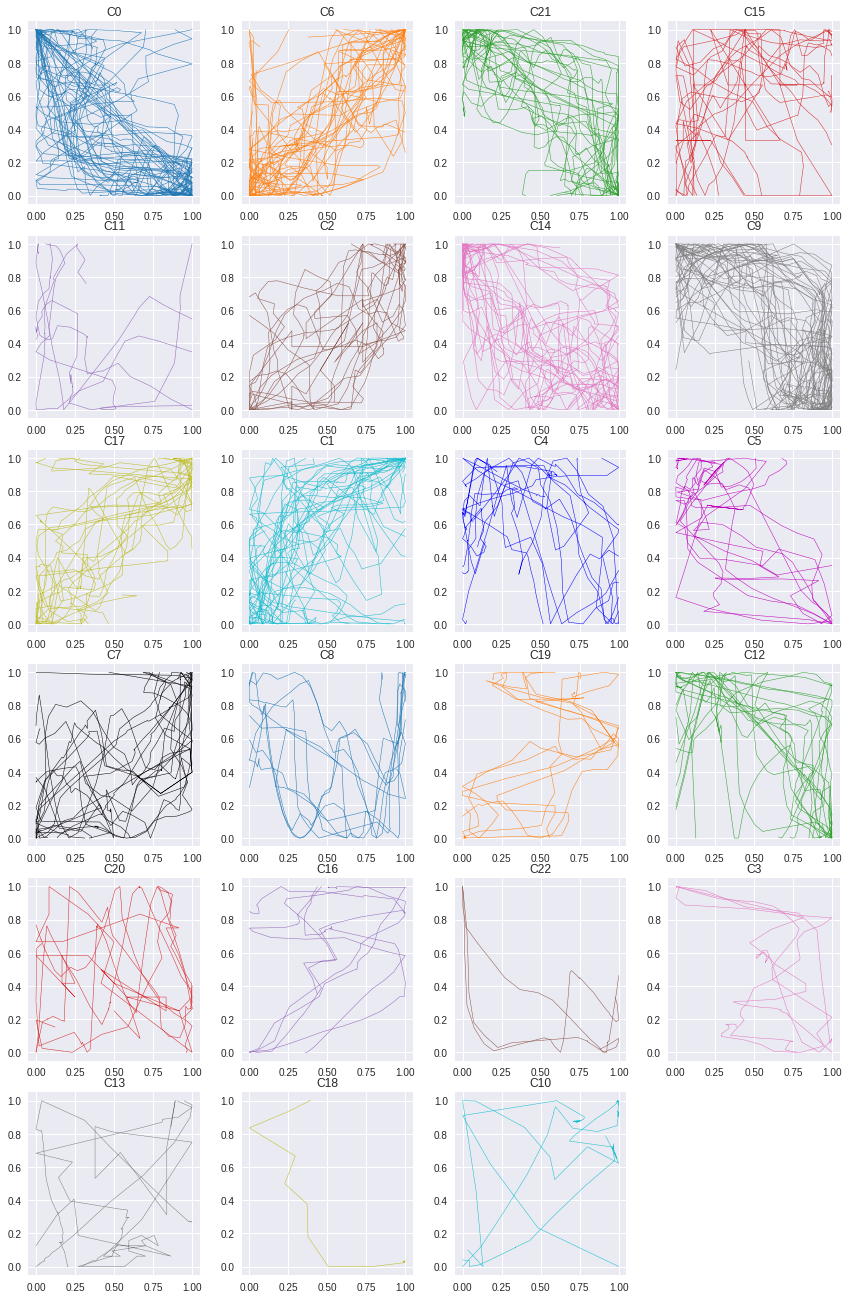
\includegraphics[width=\linewidth]{figs/clusters/CLU_H_ALL[Ed].png}
    \caption{Euclidean}
  \end{subfigure}
  \hspace{.5em}
   \begin{subfigure}[c]{0.3\linewidth}
     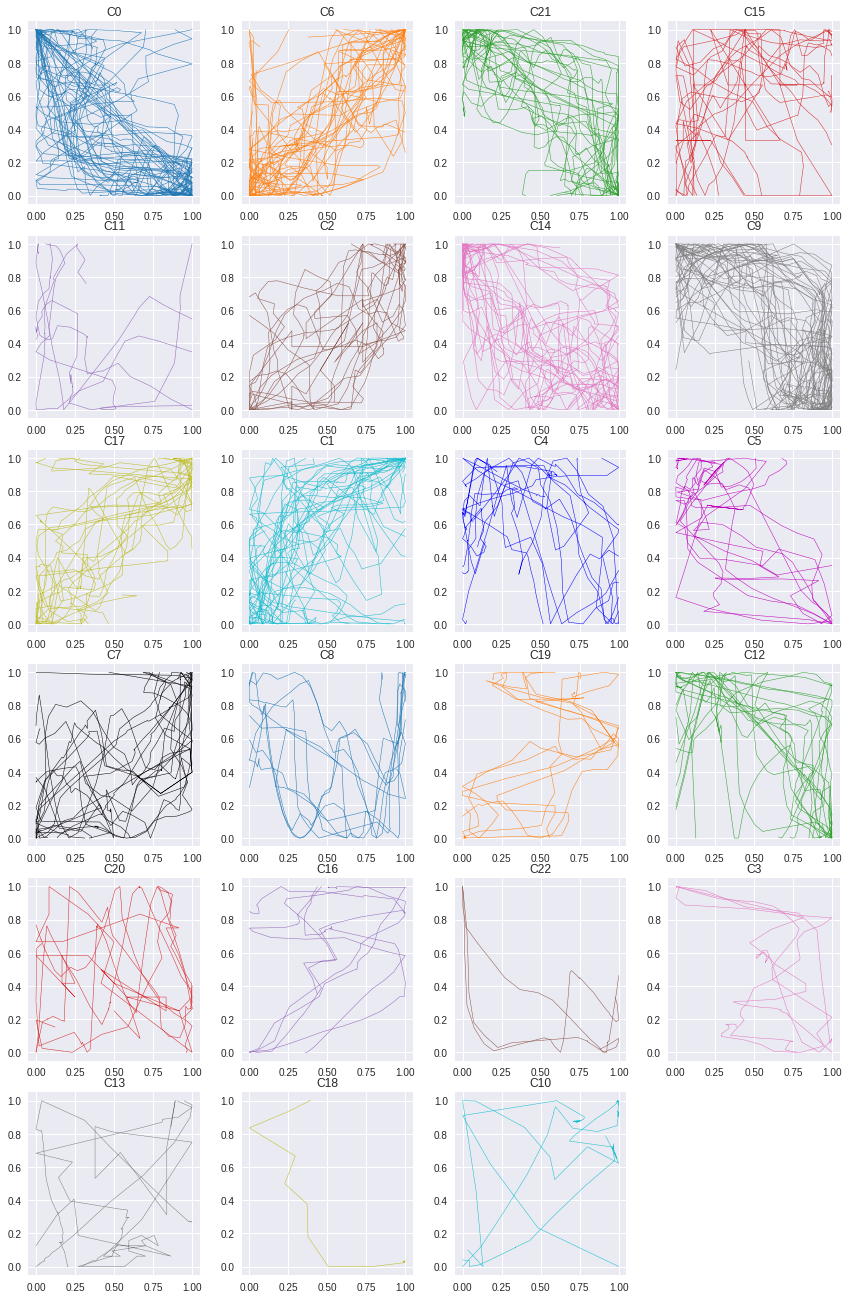
\includegraphics[width=\linewidth]{figs/clusters/CLU_H_ALL[MSM;c=1].png}
    \caption{MSM; cost=1}
  \end{subfigure}
  \hspace{.5em}
    \begin{subfigure}[c]{0.3\linewidth}
     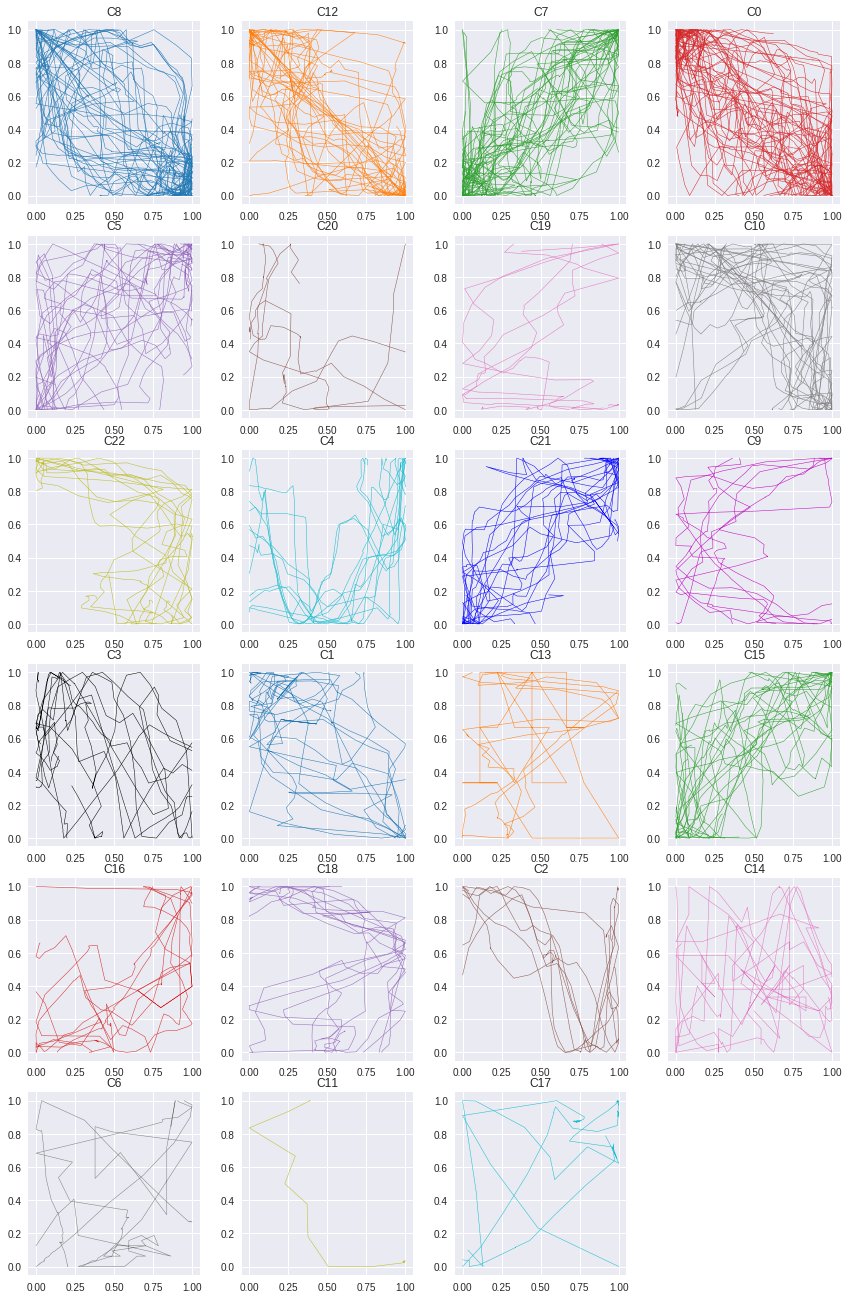
\includegraphics[width=\linewidth]{figs/clusters/CLU_H_ALL[ERP;g=0,0].png}
    \caption{ERP}
  \end{subfigure}
  \caption{Clusters of the measures that had the same raking of most similar pairs. The top row is the affinity propagation Clusters and the bottom ones are from hierarchical clustering}
  \label{fig:cluster-ed-erp-msm}
\end{figure}



\begin{figure}[h]
  \centering
  \hspace{.5em}
   \begin{subfigure}[c]{0.35\linewidth}
     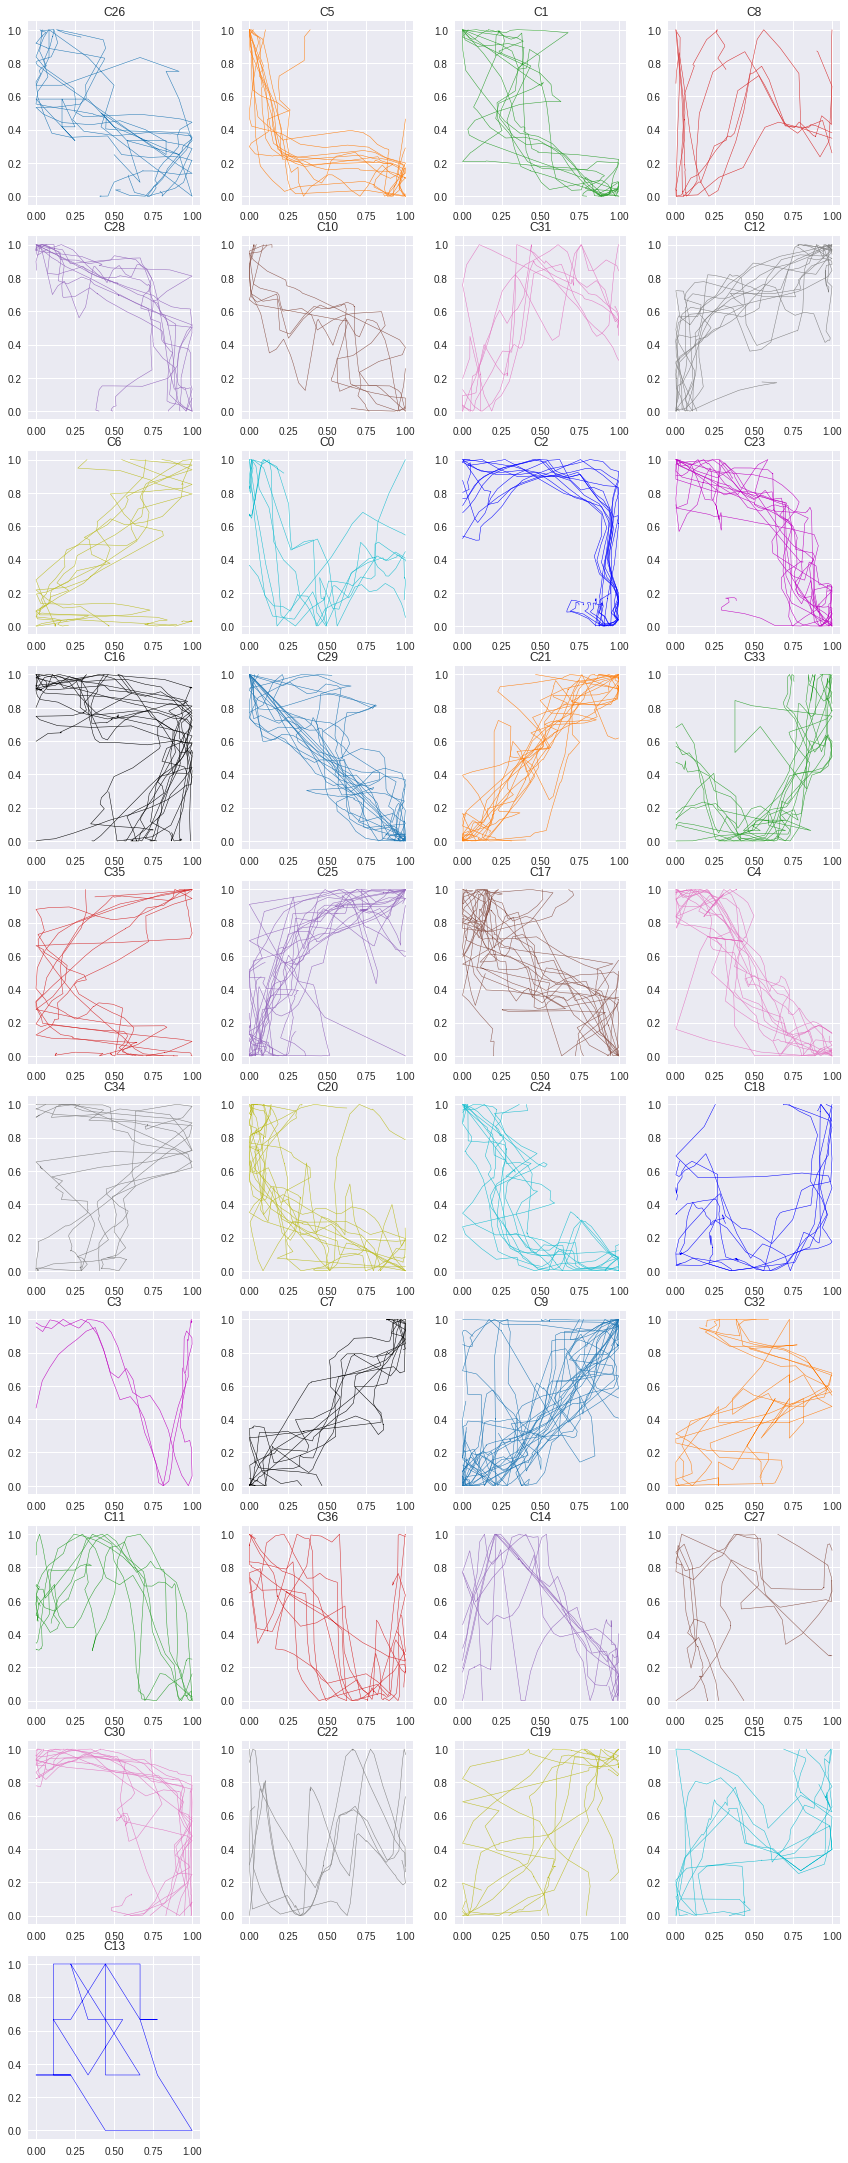
\includegraphics[width=\linewidth]{figs/clusters/CLU_AP_ALL[MSM;c=.1].png}
    \caption{MSM; Cost = 0.1}
  \end{subfigure}
  \hspace{.5em}
    \begin{subfigure}[c]{0.35\linewidth}
      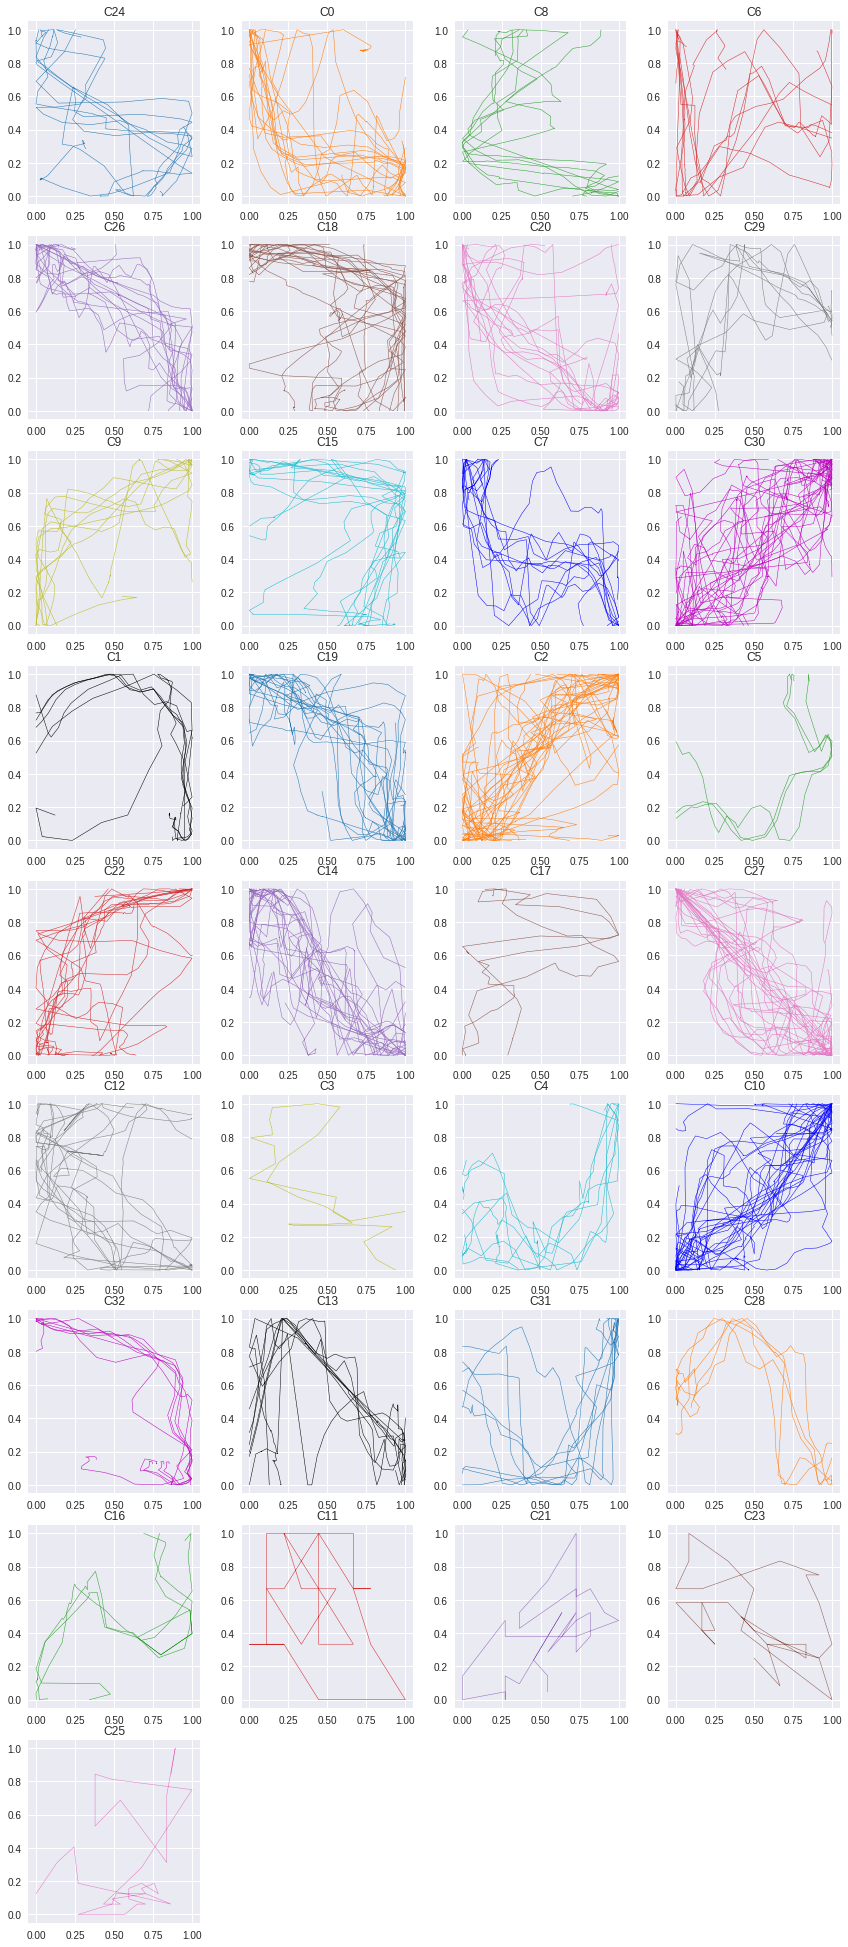
\includegraphics[width=\linewidth]{figs/clusters/CLU_AP_ALL[MSM;c=.01].png}
    \caption{MSM; Cost = 0.01}
  \end{subfigure}
  \hspace{.5em}
  
  \begin{subfigure}[c]{0.35\linewidth}
     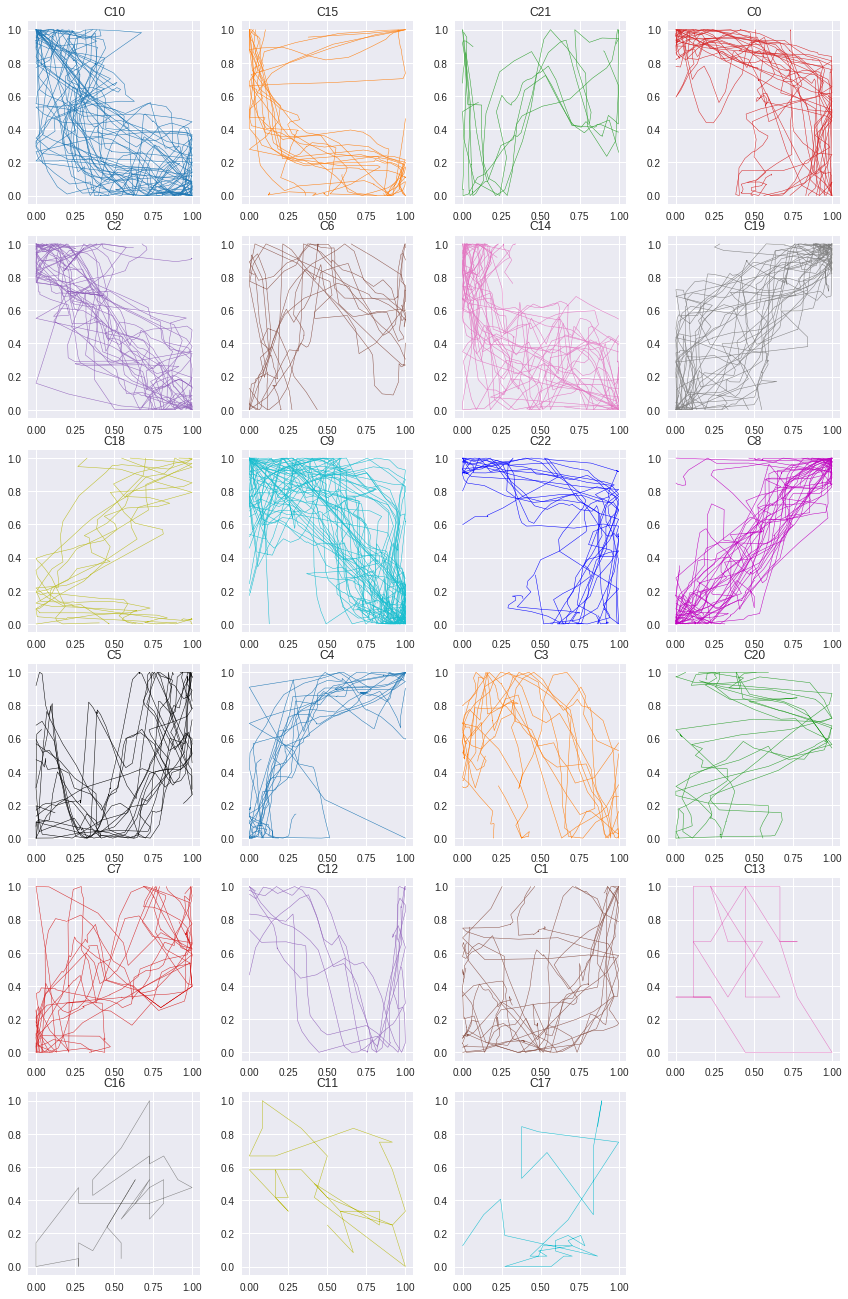
\includegraphics[width=\linewidth]{figs/clusters/CLU_H_ALL[MSM;c=.1].png}
    \caption{MSM; Cost = 0.1}
  \end{subfigure}
  \hspace{.5em}
    \begin{subfigure}[c]{0.35\linewidth}
      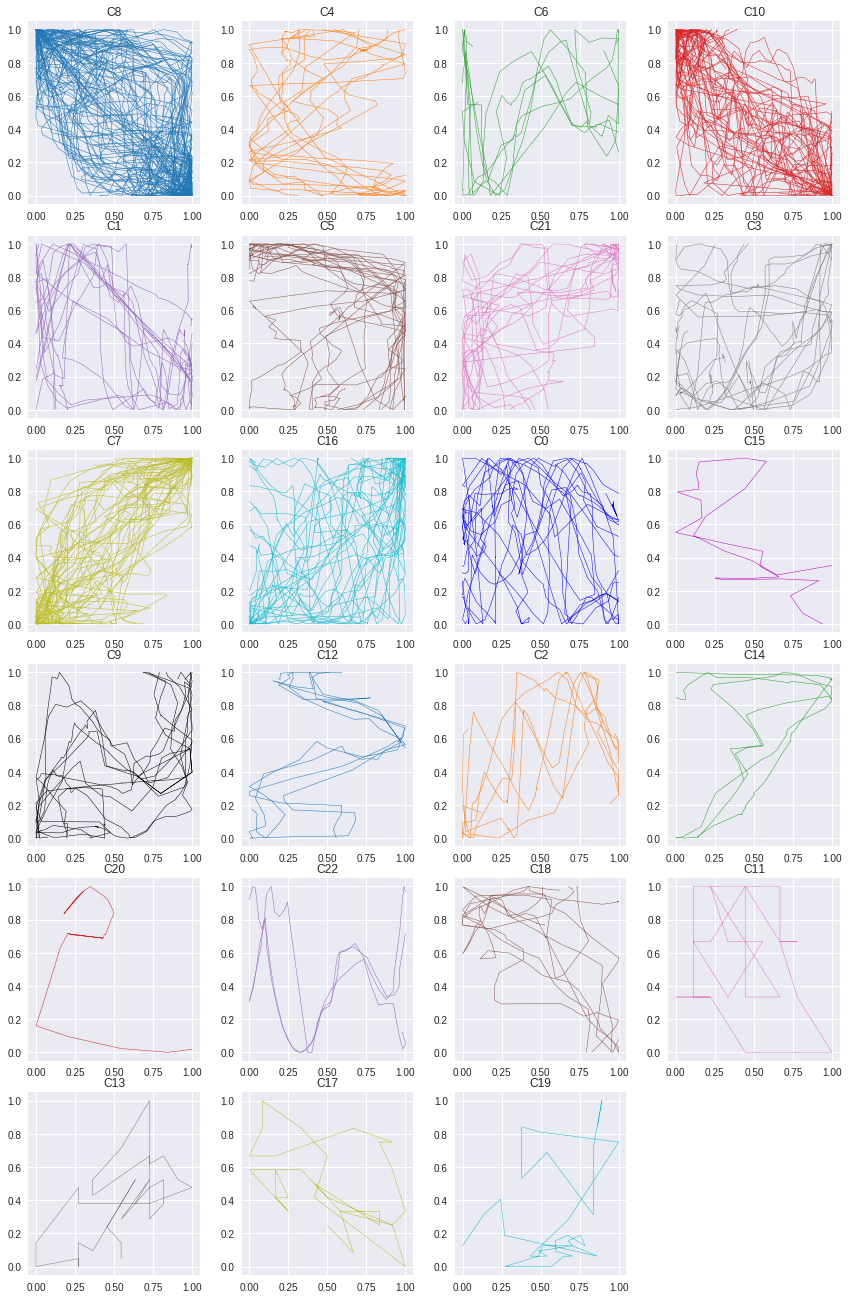
\includegraphics[width=\linewidth]{figs/clusters/CLU_H_ALL[MSM;c=.01].png}
    \caption{MSM; Cost = 0.01}
  \end{subfigure}
  
  \caption{Clusters generated by Move-Split-Merge with different parameter values.The top row is the affinity propagation Clusters and the bottom ones are from hierarchical clustering}
  \label{fig:cluster-msm}
\end{figure}


\begin{figure}[h]
  \centering
  \hspace{.5em}
   \begin{subfigure}[c]{0.35\linewidth}
     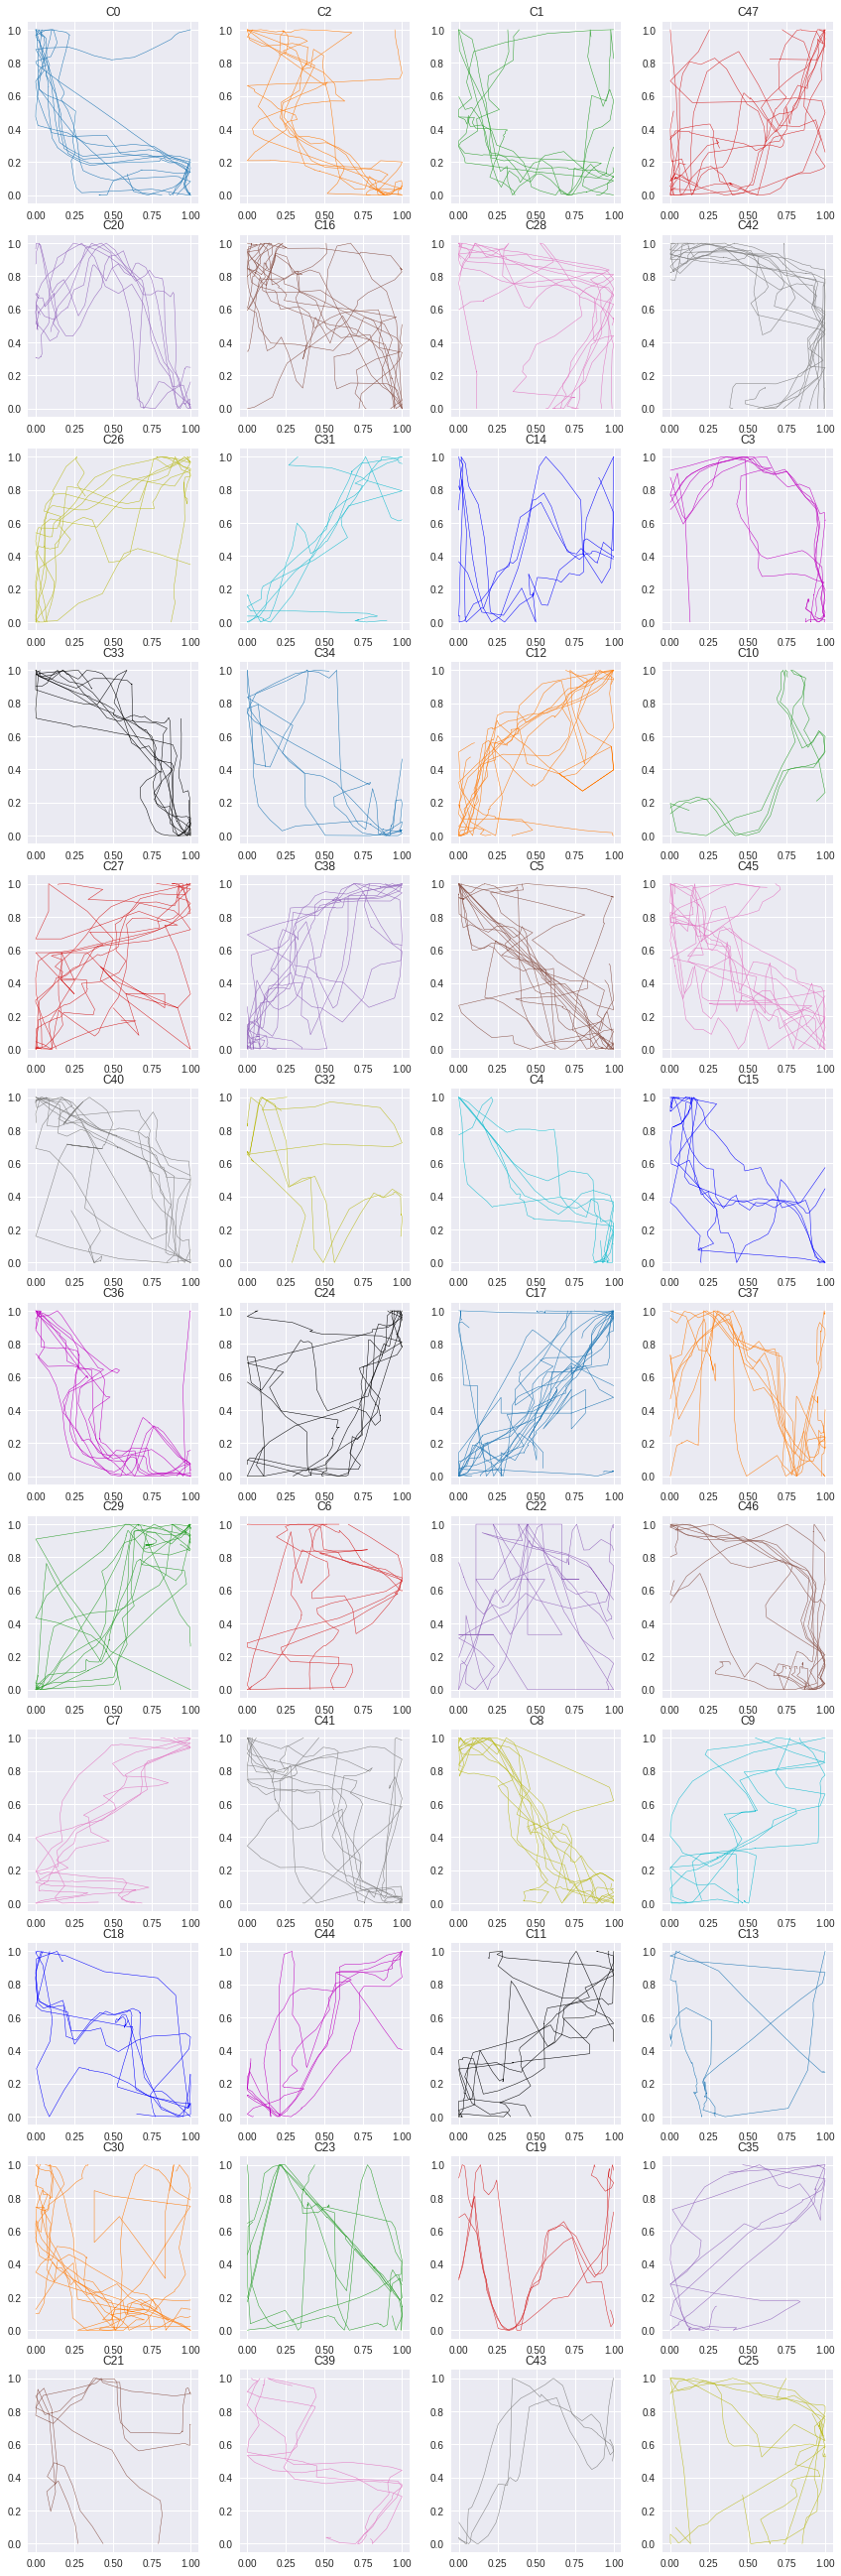
\includegraphics[width=\linewidth]{figs/clusters/CLU_AP_ALL[EDR;e=.101].png}
    \caption{EDR; $\epsilon=.101$}
  \end{subfigure}
  \hspace{.5em}
    \begin{subfigure}[c]{0.35\linewidth}
      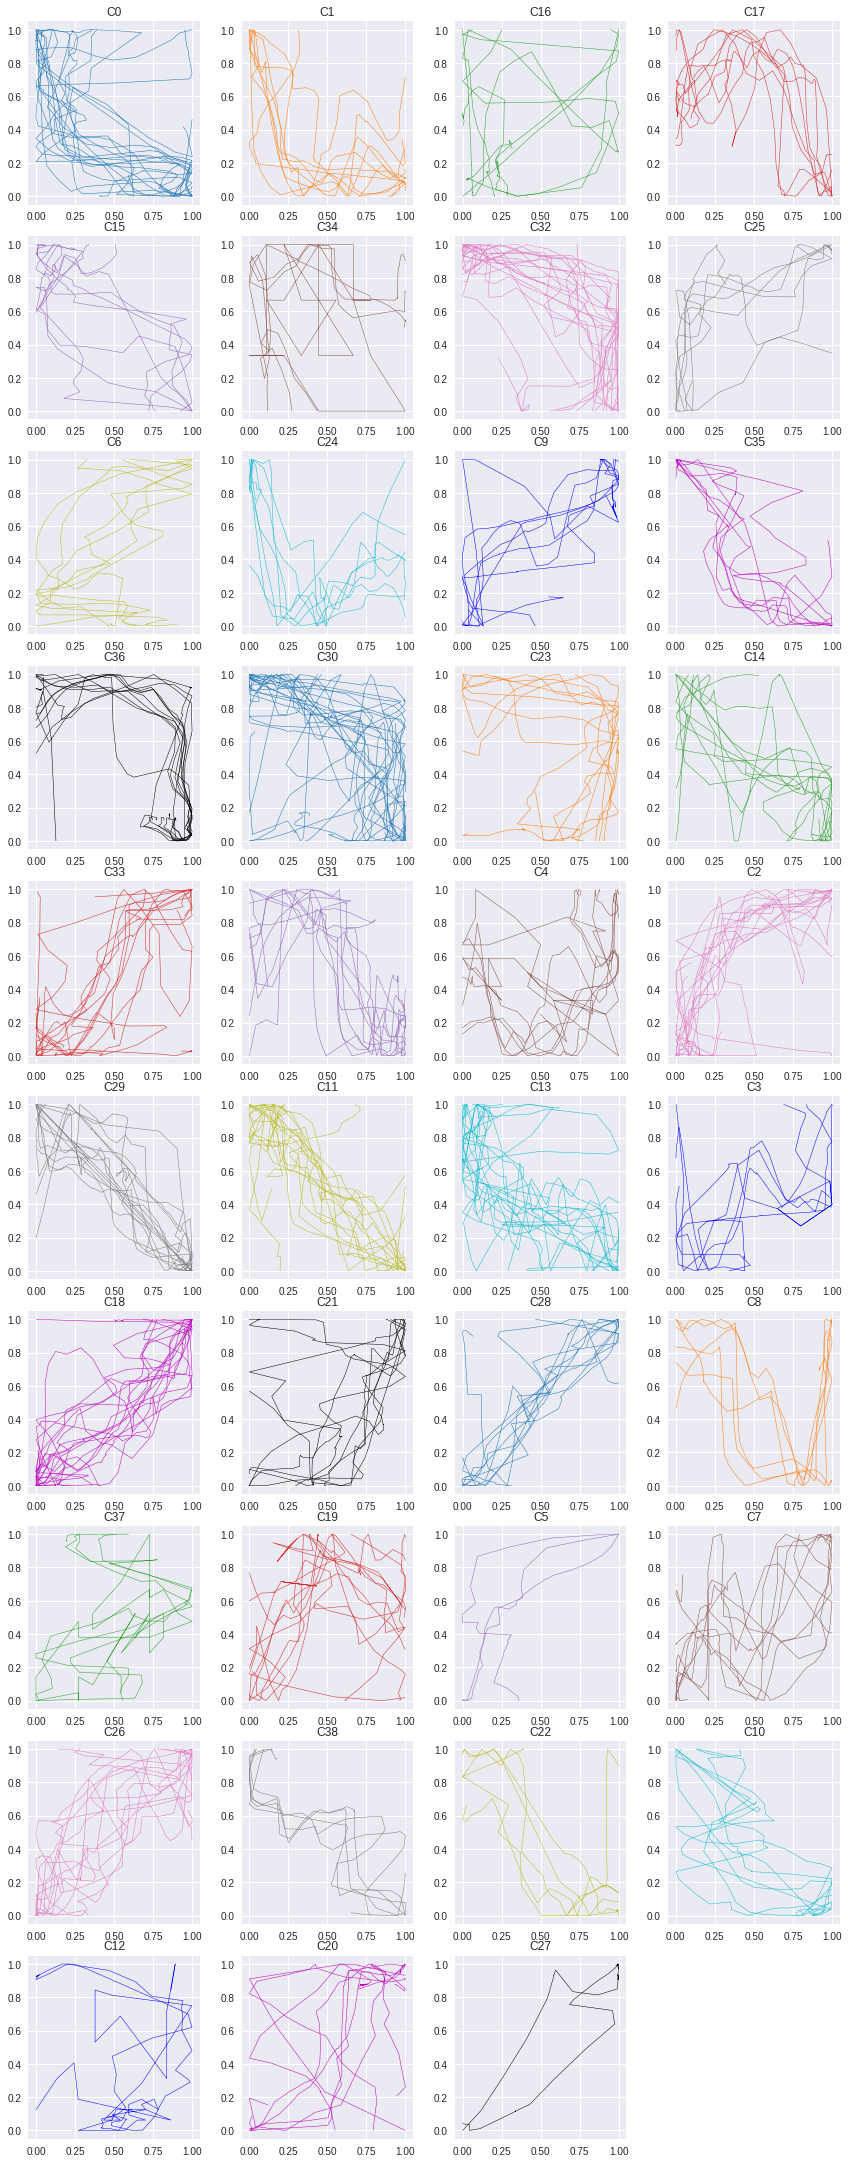
\includegraphics[width=\linewidth]{figs/clusters/CLU_AP_ALL[EDR;e=.203].png}
    \caption{EDR; $\epsilon=.203$}
  \end{subfigure}
  \hspace{.5em}
  
  \begin{subfigure}[c]{0.35\linewidth}
     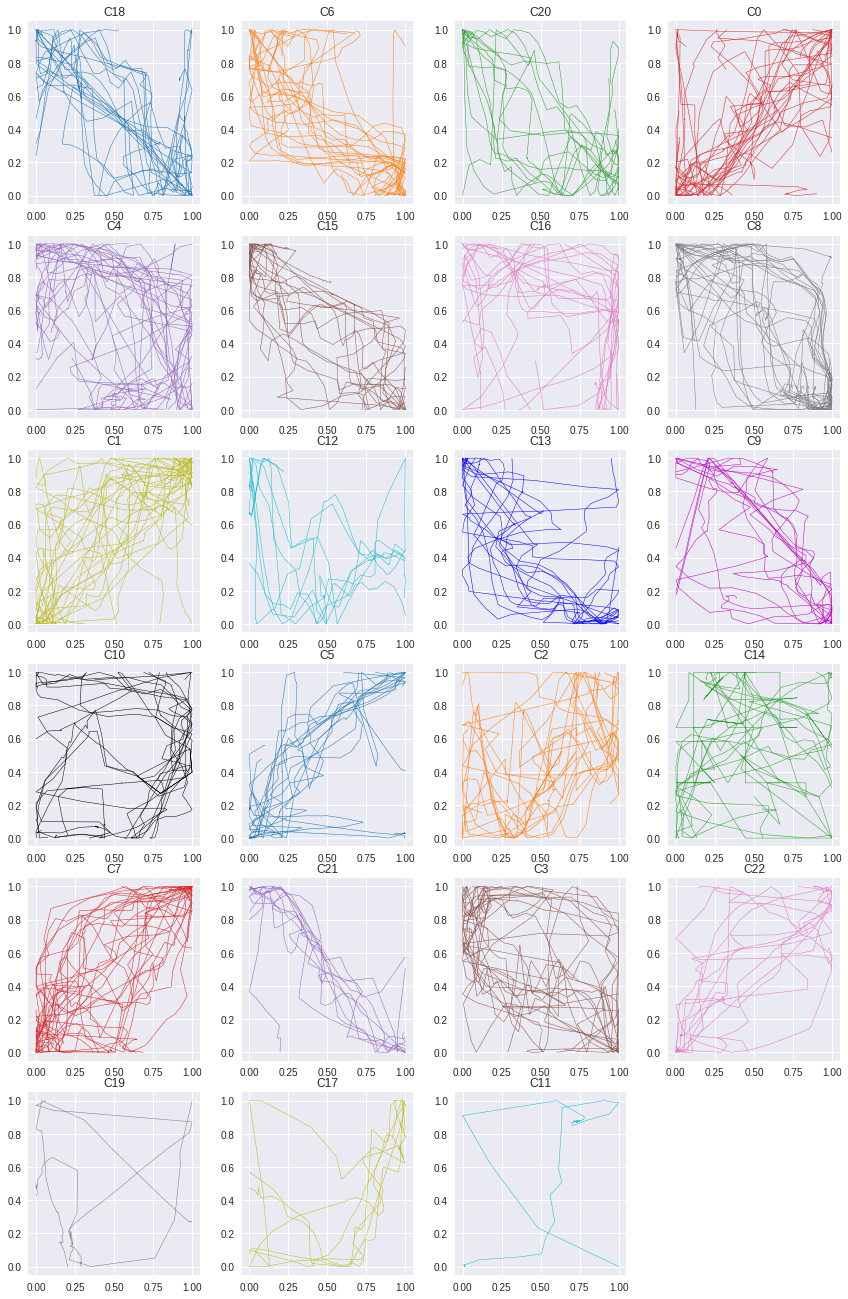
\includegraphics[width=\linewidth]{figs/clusters/CLU_H_ALL[EDR;e=.101].png}
    \caption{EDR; $\epsilon=.101$}
  \end{subfigure}
  \hspace{.5em}
    \begin{subfigure}[c]{0.35\linewidth}
      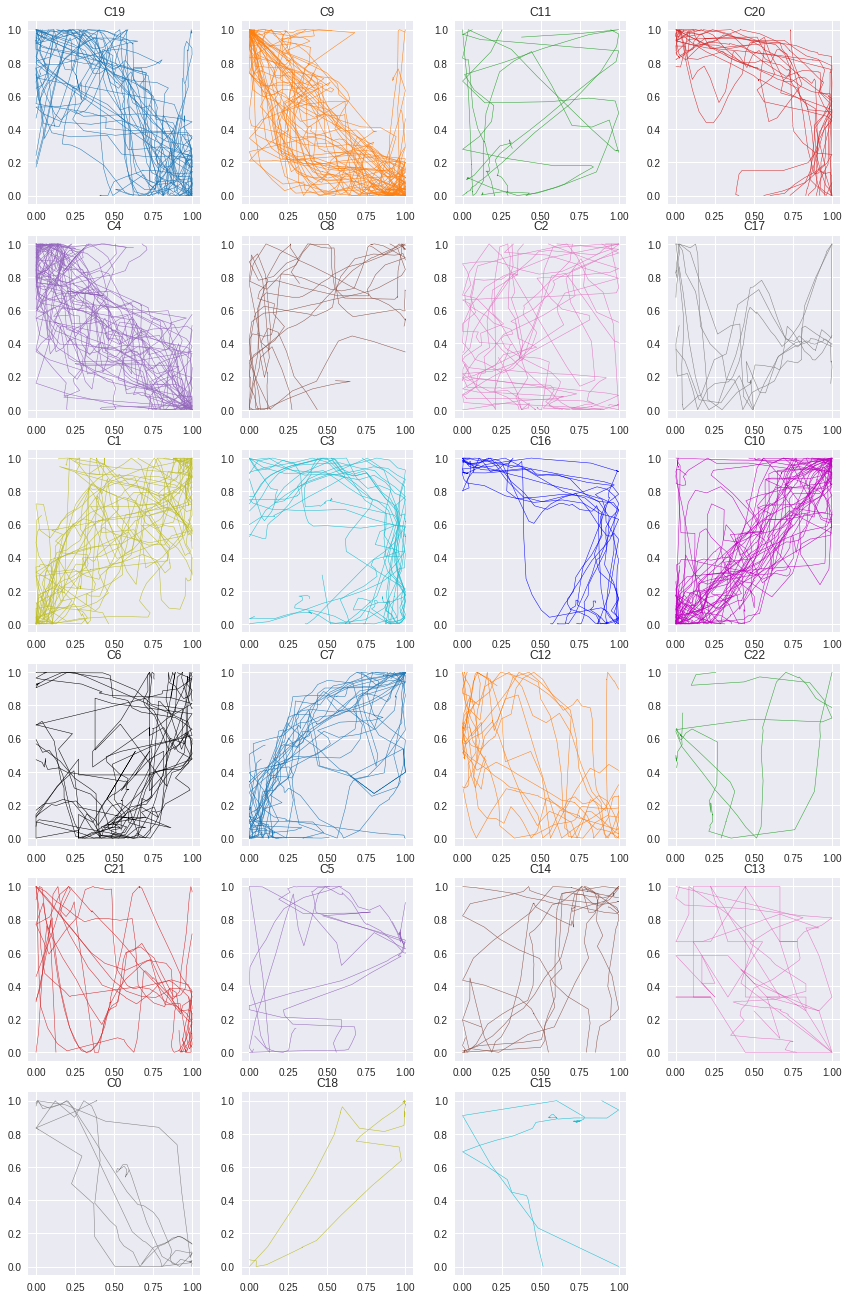
\includegraphics[width=\linewidth]{figs/clusters/CLU_H_ALL[EDR;e=.203].png}
    \caption{EDR; $\epsilon=.203$}
  \end{subfigure}
  \hspace{.5em}
 
  \caption{Clusters generated by Edit Distance on Real Sequence with different parameter values.The top row is the affinity propagation clusters and the bottom ones are from hierarchical clustering}
  \label{fig:cluster-edr}
\end{figure}



\begin{figure}[h]
  \centering
  \begin{subfigure}[c]{0.3\linewidth}
    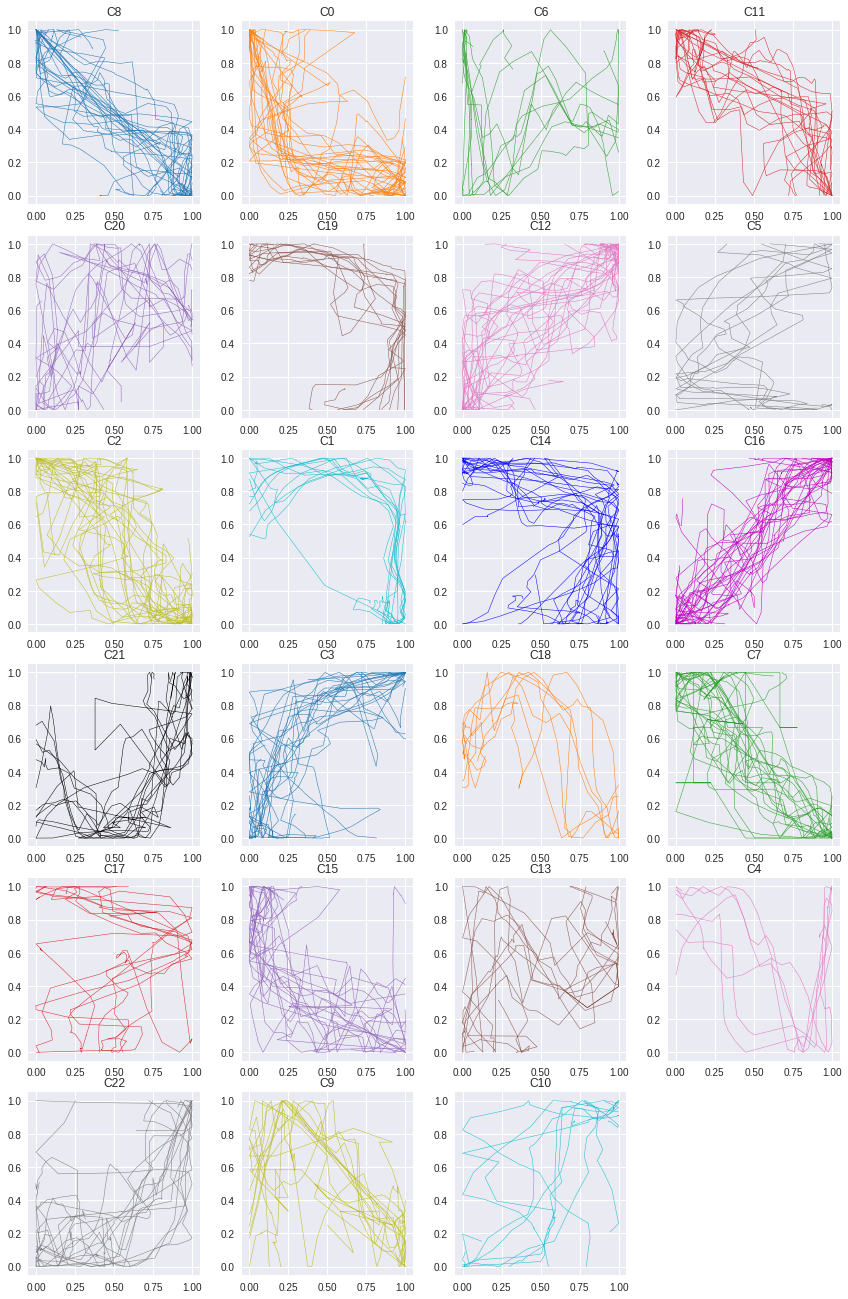
\includegraphics[width=\linewidth]{figs/clusters/CLU_AP_ALL[DTW].png}
    \caption{DTW}
  \end{subfigure}
  \hspace{.5em}
   \begin{subfigure}[c]{0.3\linewidth}
     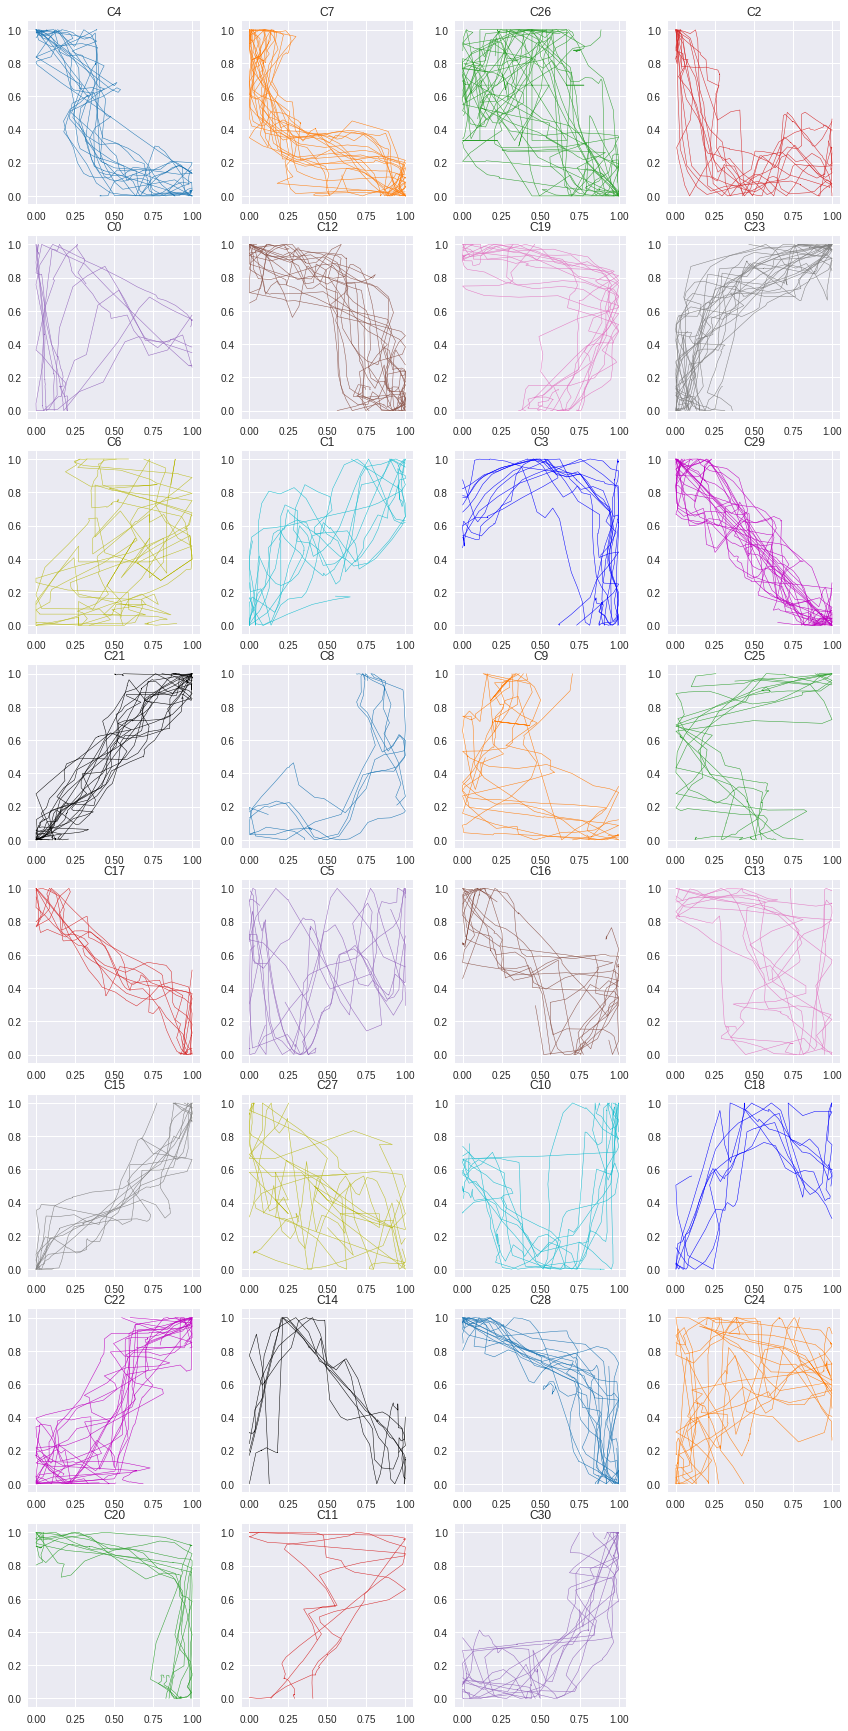
\includegraphics[width=\linewidth]{figs/clusters/CLU_AP_ALL[Hd].png}
    \caption{Hausdorff}
  \end{subfigure}
  \hspace{.5em}
    \begin{subfigure}[c]{0.3\linewidth}
     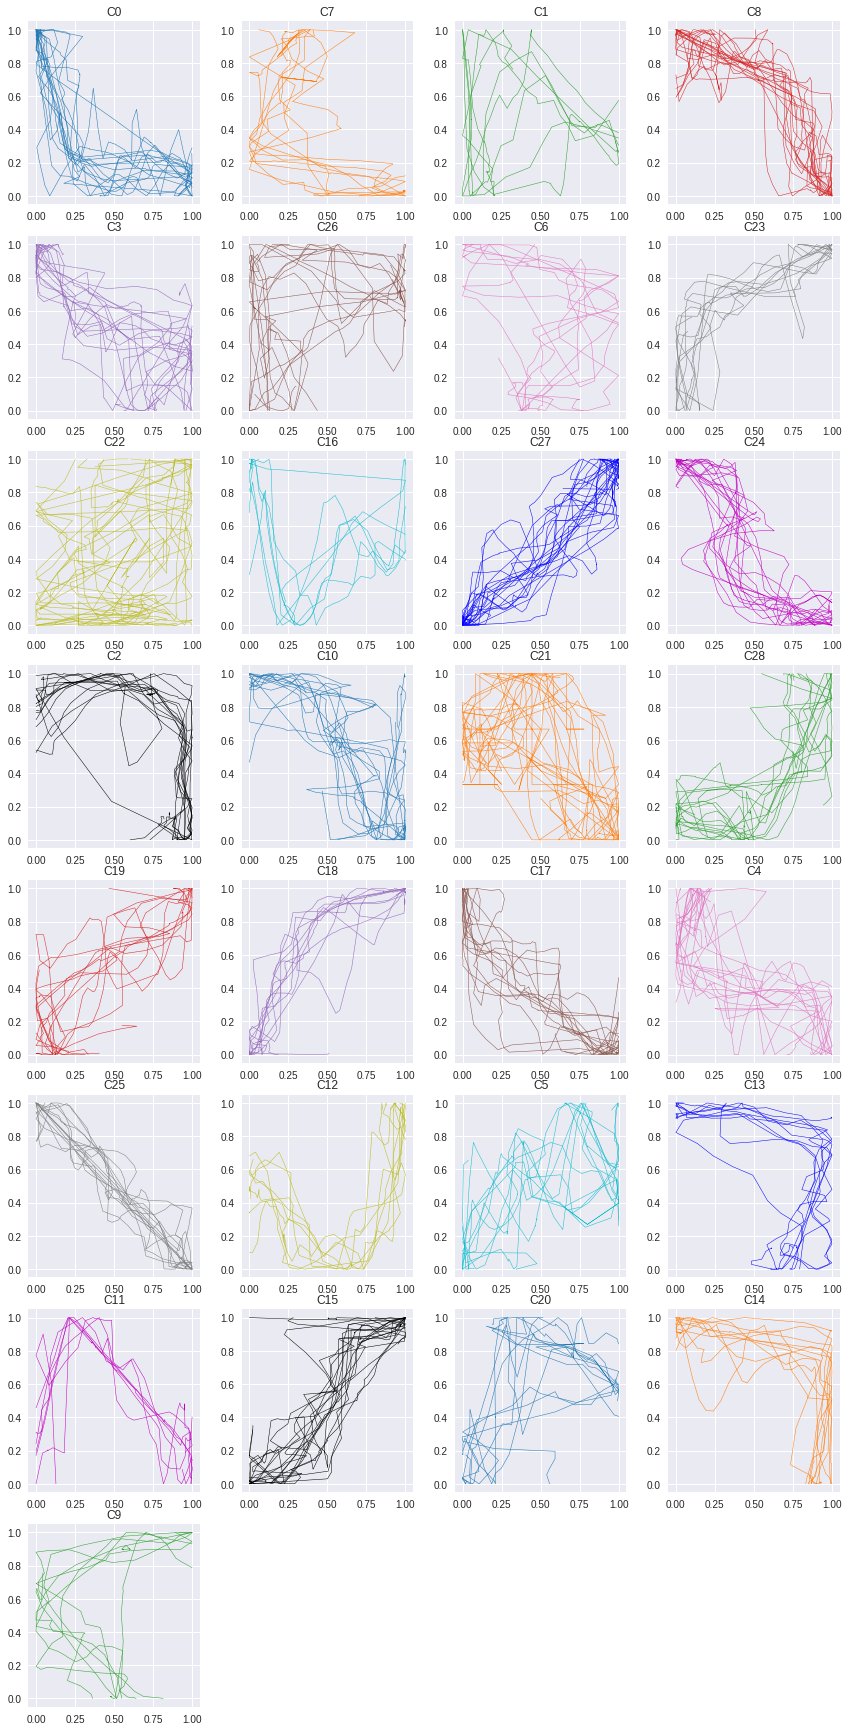
\includegraphics[width=\linewidth]{figs/clusters/CLU_AP_ALL[SSPD].png}
    \caption{SSPD}
  \end{subfigure}
  \hspace{.5em}
  \begin{subfigure}[c]{0.3\linewidth}
    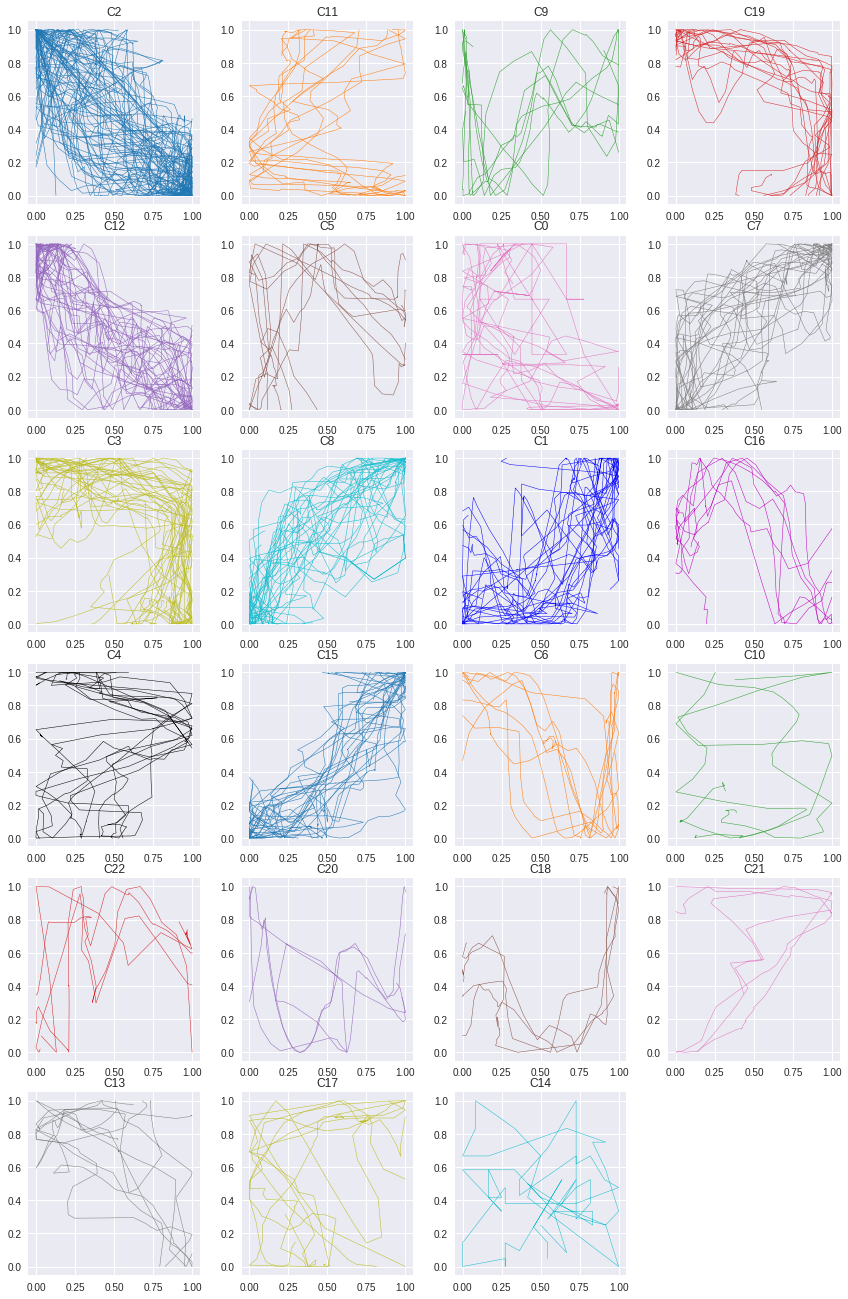
\includegraphics[width=\linewidth]{figs/clusters/CLU_H_ALL[DTW].png}
    \caption{DTW}
  \end{subfigure}
  \hspace{.5em}
   \begin{subfigure}[c]{0.3\linewidth}
     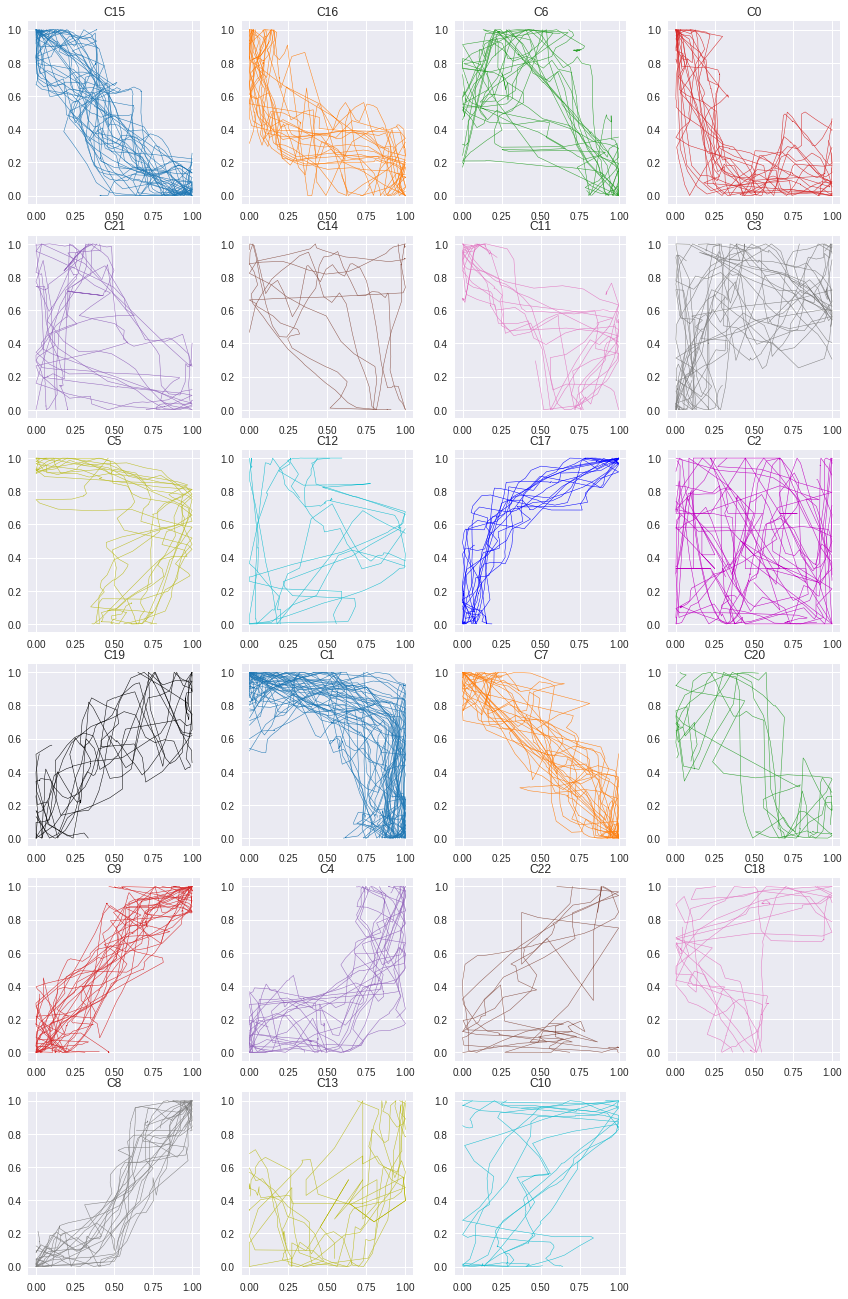
\includegraphics[width=\linewidth]{figs/clusters/CLU_H_ALL[Hd].png}
    \caption{Hausdorff}
  \end{subfigure}
  \hspace{.5em}
    \begin{subfigure}[c]{0.3\linewidth}
     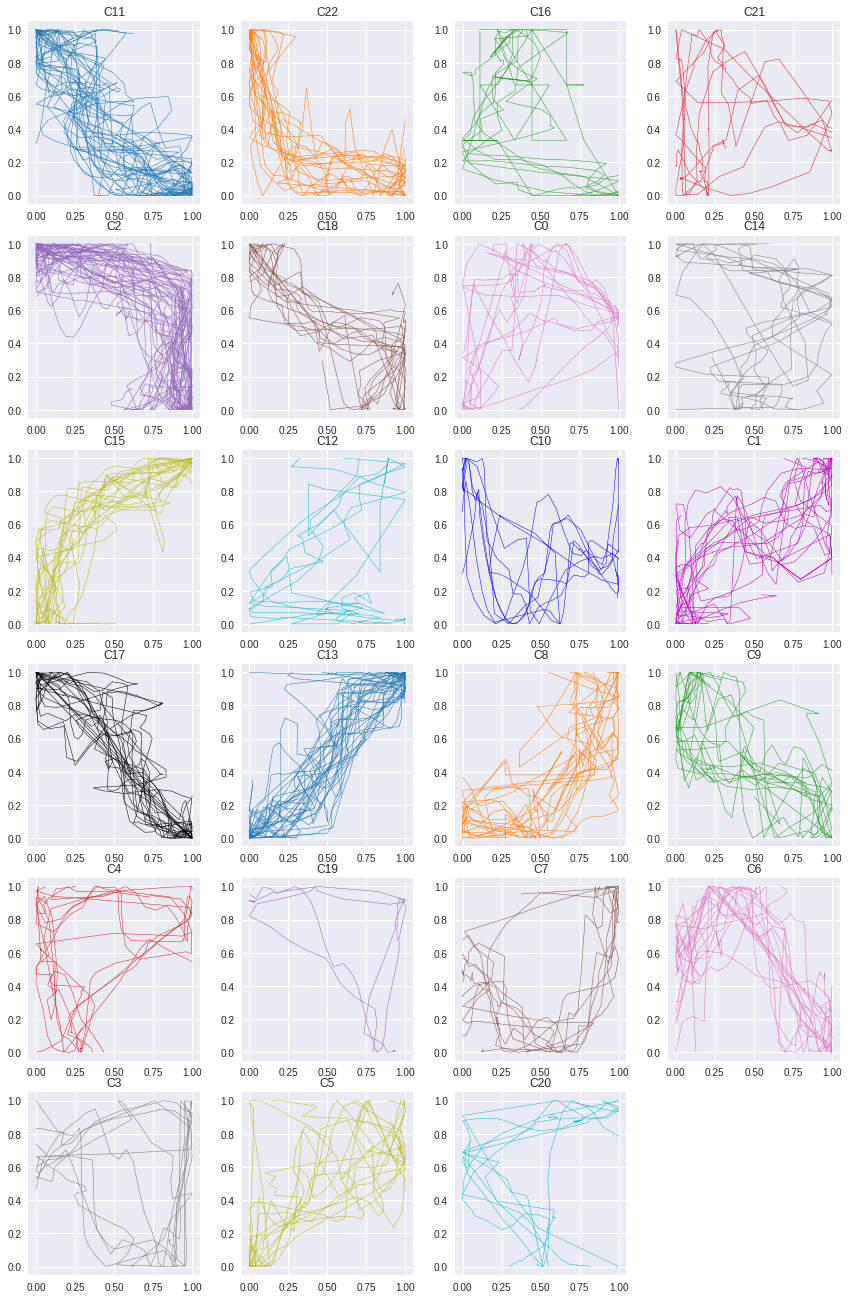
\includegraphics[width=\linewidth]{figs/clusters/CLU_H_ALL[SSPD].png}
    \caption{SSPD}
  \end{subfigure}
  \caption{Clusters created with DTW, Hausdorff and SSPD. The top row is the affinity propagation clusters and the bottom ones are from hierarchical clustering}
  \label{fig:cluster-dtw-hd-sspd}
\end{figure}




% TABLE X contains the Davies-Bouldin results of each for each cluster per type of clustering method.
% We note that SSPD and HD have resulted in the least clear clusterings using both the agglomerative hierarchical method and affinity propagation. 

% As elaborated upon in CHAPTER, human discretion remains one of the key ways to evaluate clustering task results [79]. Figures [A-Z]  are the graphical representations of the clustering results of the two best and two worst measures for each clustering technique. 


% \begin{figure}[h]
%   \centering
%   \begin{subfigure}[c]{0.35\linewidth}
%     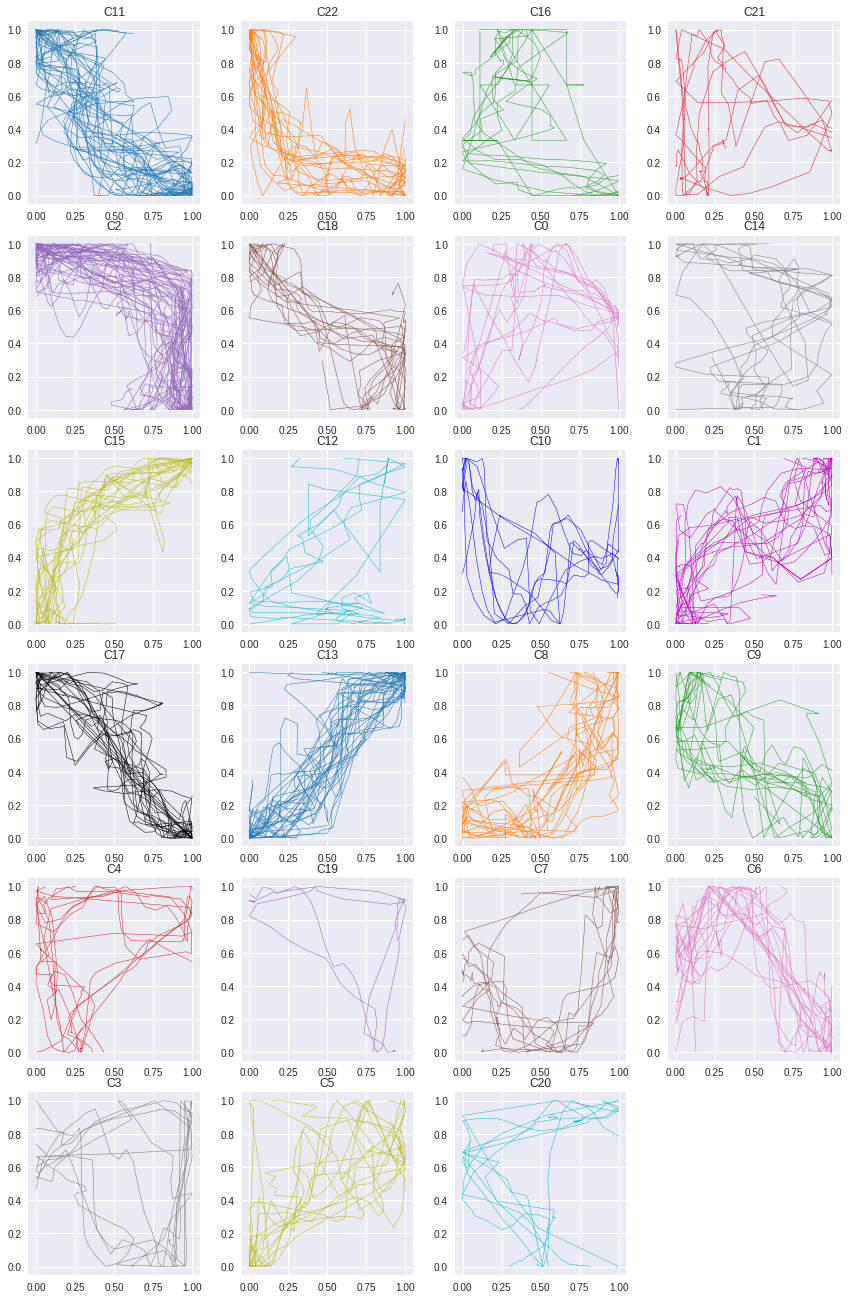
\includegraphics[width=\linewidth]{figs/clusters/CLU_H_ALL[SSPD].png}
%     \caption{Symmetric Segment Path Distance}
%   \end{subfigure}
%   \hspace{1em}
%   \begin{subfigure}[c]{0.35\linewidth}
%      \includegraphics[width=\linewidth]{figs/clusters/CLU_H_ALL[HD].png}
%     \caption{Hausdorff Distance }
%   \end{subfigure}
%   \caption{Final HCA-Clusters of the measures the worst Davies-Bouldin Index}
%   \label{fig:cluster-h-worst}
% \end{figure}

% For the sake of brevity, only a handful of the clustering are shown in detail and the remaining graphical representations are found in the APPENDIX. 
% Figures [A-Z] are the graphical representations of the clustering results of the two best and two worst measures for each clustering technique. 
